Up to this point the actual layout of data in memory has been treated in a somewhat abstract manner, with no detail about how it is actually implemented in \neuron.
For example, the pseudo-code examples have treated the data for each mechanism as though it was stored as a \emph{structure of arrays} (SoA), when it is actually stored as an \emph{array of scructures}.

Here we will describe the data layout as it is currently implemented. Before generalizing the storage, and suggesting optimization strategies, we want to understand the current data model, and all of the use cases that it must support.

\begin{note}
A good spot to start refactoring would be a simple serialization framework for reading and writing the state of a cell group in \neuron. This would be a good exercise in getting into the nitty-gritty of the memory layout, and could be used as input data for unit tests when trying out new approaches.
\end{note}

%%%%%%%%%%%%%%%%%%%%%%%%%%%%%%%%%%%%%%%%%%%%%%%%%%%%%%%%%%%%%%%%%%%%%%%%%%%%%%
\subsection{Parallel Data Distribution}
%%%%%%%%%%%%%%%%%%%%%%%%%%%%%%%%%%%%%%%%%%%%%%%%%%%%%%%%%%%%%%%%%%%%%%%%%%%%%%
Each neuron cell is represented as of a tree of nodes, as illustrated in \fig{fig:tree}.
The properties of individual cells, including the number of nodes and the type, number and distribution of synapses, vary significantly.
These properties affect the computational resources required to perform a time step for a cell, e.g. cells with more synapses require more expensive \lst{state} and \lst{current} computations.
The number and type of mechanisms in a cell can be used as an \textit{a-priori estimate} its computational complexity.

To ensure load balancing, cells are organized into groups that have roughly equivalent computational overheads during circuit generation.
As a result, some cell groups have more cells than others to ensure that total computational effort required per group is balanced.
Each group of cells is stored in a separate \file{.dat} file, which are then distributed in a round-robin fashion when simulation data is loaded in \lst{nrn_setup}.

Parallelism is implemented distributing the cells, with individual cells processed serially.
There are two levels of parallelism:
\begin{enumerate}
\item
    \textbf{MPI (course-grained)}: the cell groups are distributed between MPI ranks.
\item
    \textbf{Thread (fine-grained)}: each cell group on an MPI rank is assigned to a thread.
\end{enumerate}
Threading is performed using pthreads, with explicit communication of spike information between both threads and MPI processes.
Each cell group is stored in a \lst{NrnThread} data structure (see \fig{lst:NrnThreadInfo}), which is named as such because each cell group is assinged to a thread (the name should be changed to better represent the data).

\begin{note}
The fine fine-grained parallelism could be implemented on a finer scale than it currently is, i.e. with multiple threads processing each cell group/cell. There was a CUDA implementation of Neuron that took this approach, and on the GPU this is probably necessary to expose enough parallelism. There have been some successful tests on the Xeon Phi where each thread was assigned a cell group.
\end{note}
%%%%%%%%%%%%%%%%%%%%%%%%%%%%%%%%%%%%%%%%%%%%%%%%%%%%%%%%%%%%%%%%%%%%%%%%%%%%%%
\subsection{Cell Groups}
%%%%%%%%%%%%%%%%%%%%%%%%%%%%%%%%%%%%%%%%%%%%%%%%%%%%%%%%%%%%%%%%%%%%%%%%%%%%%%
The cells in a cell group are ``flattened'' together in the \lst{NrnThread} data structure, i.e. individual cells are not stored seperately.
As an example, for the TEST2 dataset distributed with the PCP:
    \begin{itemize}
    \item
        there are around 60--70 cells per cell group.
    \item
        each cell has of the order 400--450 nodes.
    \item
        each cell group has 25,000--30,000 nodes in total.
    \end{itemize}
    The cells are packed together with all node and mechanism data for all nodes in all cells in the cell group packed into flat arrays.
        Given $n_c$ cells in the cell group with a total of $n$ nodes, the root nodes are indexed \lst{[1:n_c]}, and the rest of the nodes are indexed \lst{[n_c+1:n]}\footnote{This is evident in the loops over \lst{child_nodes=ncells+1:nnondes} and \lst{1:ncells}}.

%-----------------------------------------------------------------------------
\begin{note}
Storing the cells in the cell group as such means that all of the steps in a timestep in \fig{fig:timestepDiagram} are applied to the entire cell group, not to individual cells.
This ignores the fact that the cells can be integrated in time independently, with coordination only required when communicating spike events.
An obvious approach for introducing more fine-grained parallelism is to distriubute individual cells, not cell groups, between threads.
This approach exposes more work that can be performed in parallel, however, it has load balancing issues, because of the variation in complexity between indivdual cells.
\end{note}
%-----------------------------------------------------------------------------

The main storage requirements for a mechanism are storing the vectors relating to the linear system and the vectors that describe mechanism state.
These vectors are not allocated separately, instead a single memory buffer is allocated (\lst{NrnThread::data[]}), and the vector pointers point to sub-arrays in \lst{NrnThread::data[]}
\footnote{
Allocating memory in one large block is more memory efficient than allocating many smaller vectors with individual calls to \lst{malloc}.
}.
This process of allocating the memory is performed in the function \lst{read_phase2} in \file{nrniv/nrn_setup.cpp}.

The layout of vectors in the \lst{data[]} array is shown in \fig{}.
When the cell group is read from file, the total size of the \lst{data[]} array is determined, then the memory allocated.
The vectors that describe the linear system and the area of each node, \lst{[VEC_RHS, VEC_D, VEC_A, VEC_B, VEC_V, actual_area]}, are placed at the front of the data vector.
The state data for the mechanism then follows.

%------------------------------------------------------------------
\begin{figure}[htp!]
\documentclass[tikz,border=10pt]{standalone}

\usepackage{tikz}
\usetikzlibrary{positioning}
\usetikzlibrary{shapes,arrows,backgrounds,fit,shapes.geometric,calc}
\usetikzlibrary{pgfplots.groupplots}
\usepackage{pgfplots}
\usepackage{pgfplotstable}
\usepackage{listings}
\usepackage{lstautogobble}
\usepackage{color}

\lstset{
    language=[ANSI]C++,
    basicstyle=\small\ttfamily,
    identifierstyle=\color{black}\small\ttfamily,
    keywordstyle=\color{red}\small\ttfamily,
    commentstyle=\color{green!30!black}\bf\small\ttfamily,
    breaklines=true
}

\tikzset{
    %Define standard arrow tip
    >=stealth',
    % Define arrow style
    pil/.style={
           ->,
           thick,
           shorten <=2pt,
           shorten >=2pt,}
}
\newcommand{\nodewidth}{1.1cm}
\newcommand{\mechnodewidth}{0.8cm}
\newcommand{\nodeheight}{0.75cm}
\newcommand{\lst}[1]{\lstinline!#1!}

\begin{document}
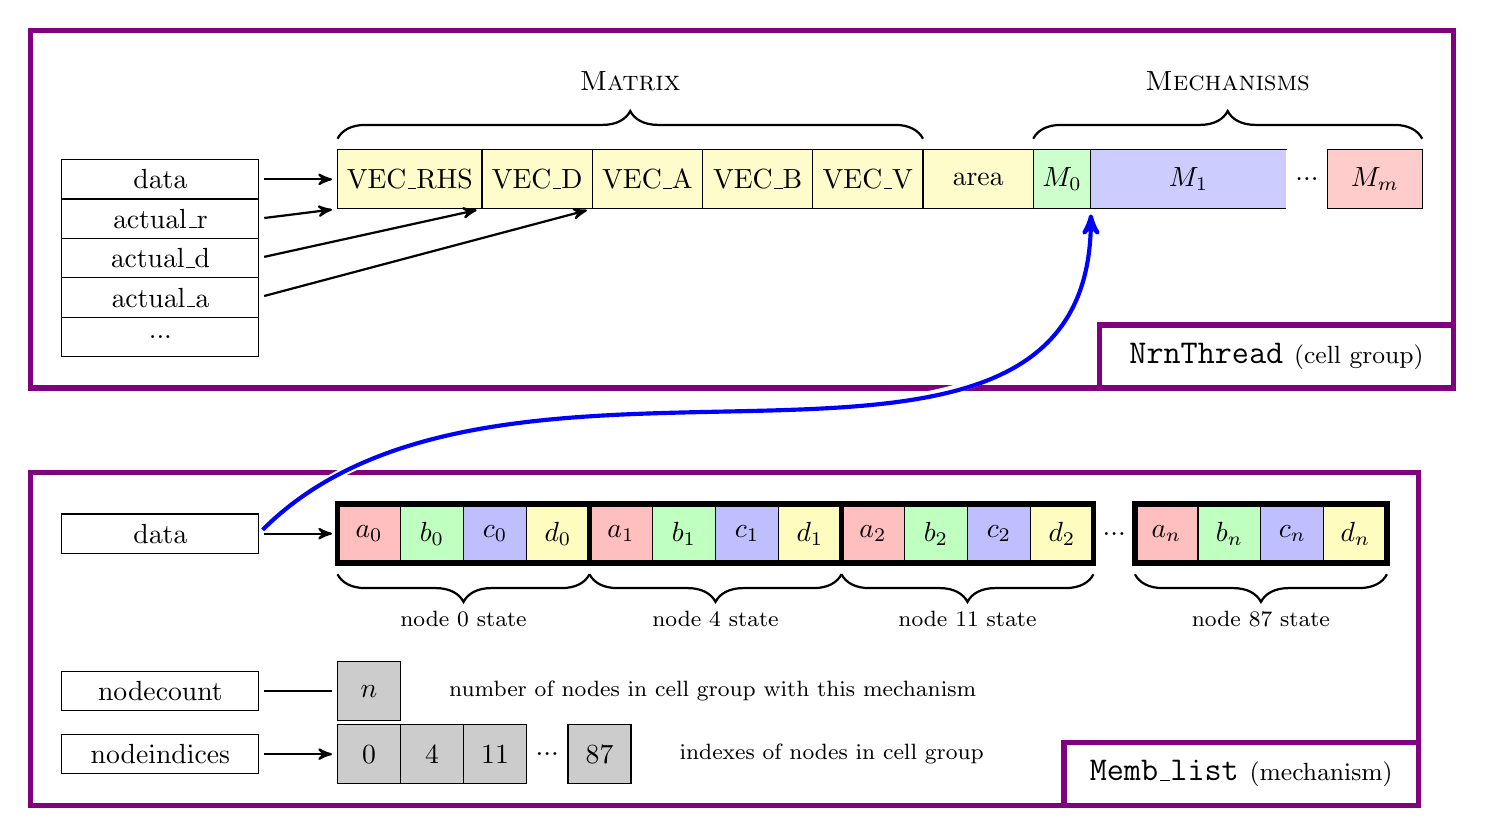
\begin{tikzpicture}[x=0cm, y=0cm, node distance=0 cm,outer sep = 0pt]
\tikzstyle{nvec}=[draw, rectangle,
                  minimum height=\nodeheight, minimum width=\nodewidth,
                  fill=yellow!20,anchor=south west,minimum width=1.4cm]
\tikzstyle{mch0}=[draw, rectangle,
                  minimum height=\nodeheight,
                  fill=green!20,anchor=south west,minimum width=0.5cm]
\tikzstyle{mch1}=[draw, rectangle,
                  minimum height=\nodeheight,
                  fill=blue!20,anchor=south west,minimum width=2.48cm]
\tikzstyle{mch2}=[draw, rectangle,
                  minimum height=\nodeheight,
                  fill=red!20,anchor=south west,minimum width=1.2cm]
\tikzstyle{blank}=[draw=none, rectangle,
                   fill=white, minimum height=\nodeheight,
                   minimum width=0.1cm, anchor=south west]
\tikzstyle{pointer}=[draw=black, fill=white, rectangle,
                   minimum height=0.5cm, minimum width=2.5cm, anchor=south west]

\tikzstyle{t0}=[draw, rectangle,  minimum height=\nodeheight, minimum width=\mechnodewidth,
                fill=red!25,anchor=south west]
\tikzstyle{t1}=[draw, rectangle,  minimum height=\nodeheight, minimum width=\mechnodewidth,
                fill=green!25,anchor=south west]
\tikzstyle{t2}=[draw, rectangle,  minimum height=\nodeheight, minimum width=\mechnodewidth,
                fill=blue!25,anchor=south west]
\tikzstyle{t3}=[draw, rectangle,  minimum height=\nodeheight, minimum width=\mechnodewidth,
                fill=yellow!25,anchor=south west]
\tikzstyle{cover}=[draw, rectangle,  minimum height=\nodeheight, minimum width=3.2cm,
                line width = 2pt,anchor=south west]
\tikzstyle{index}=[draw, rectangle,  minimum height=\nodeheight, minimum width=\mechnodewidth,
                   fill=black!20,anchor=south west]
%%%%%%%%%%%%%%%%%%%%%%%%%%%%%%%%%
% NrnThread
%%%%%%%%%%%%%%%%%%%%%%%%%%%%%%%%%
\node[pointer] (data) at (0,0)         {\lst{data}};
\node[nvec] (vecr)    [right = 1cm of data] {\lst{VEC_RHS}};

\node[nvec] (vecd)    [right = of vecr] {\lst{VEC_D}};
\node[nvec] (veca)    [right = of vecd] {\lst{VEC_A}};
\node[nvec] (vecb)    [right = of veca] {\lst{VEC_B}};
\node[nvec] (vecv)    [right = of vecb] {\lst{VEC_V}};
\node[nvec] (vecarea) [right = of vecv] {\lst{area}};
\node[mch0] (m0)      [right = of vecarea] {$M_0$};
\node[mch1] (m1)      [right = of m0] {$M_1$};
\node[blank](dd)      [right = of m1] {...};
\node[mch2] (m2)      [right = of dd] {$M_{m}$};

\node[pointer] (vecrp)[below = of data] {\lst{actual_r}};
\node[pointer] (vecdp)[below = of vecrp] {\lst{actual_d}};
\node[pointer] (vecap)[below = of vecdp] {\lst{actual_a}};
\node[pointer] (vecetc)[below = of vecap] {\lst{...}};

\path[pil,->] (data.east)  edge (vecr.west);
\path[pil,->] (vecrp.east) edge (vecr.south west);
\path[pil,->] (vecdp.east) edge (vecd.south west);
\path[pil,->] (vecap.east) edge (veca.south west);


\draw[decorate,decoration={brace,raise=4pt,amplitude=10pt},thick]
  (vecr.north west)--(vecv.north east)
  node[midway,yshift=25pt] (matbrace) {\sc Matrix};

\draw[decorate,decoration={brace,raise=4pt,amplitude=10pt},thick]
  (m0.north west)--(m2.north east)
  node[midway,yshift=25pt] (mechbrace) {\sc Mechanisms};

\tikzset{typeline/.style={draw=blue!50!red, line width=2pt,
                          inner sep=4mm, rectangle}};
\node (nrnthread)[typeline,
                  fit = (vecr)(data)(vecd)(veca)(vecb)(vecv)(vecarea)
                        (m0)(m1)(dd)(m2)
                        (matbrace)(mechbrace)
                        (vecrp)(vecap)(vecdp)(vecetc)] {};

\node at (nrnthread.south east)
    [anchor=south east, fill=white, draw=red!50!blue, line width=2pt, minimum height=0.8cm, minimum width=4.5cm]
    {\large {\texttt{NrnThread}} \small (cell group)};

%%%%%%%%%%%%%%%%%%%%%%%%%%%%%%%%%
% Memb_list
%%%%%%%%%%%%%%%%%%%%%%%%%%%%%%%%%

\node[pointer] (datamech)[below = 2cm of vecetc] {\lst{data}};
\node[t0] (m00) [right = 1cm of datamech] {$a_0$};
\node[t1] (m01) [right = of m00] {$b_0$};
\node[t2] (m02) [right = of m01] {$c_0$};
\node[t3] (m03) [right = of m02] {$d_0$};
\node[t0] (m10) [right = of m03] {$a_1$};
\node[t1] (m11) [right = of m10] {$b_1$};
\node[t2] (m12) [right = of m11] {$c_1$};
\node[t3] (m13) [right = of m12] {$d_1$};
\node[t0] (m20) [right = of m13] {$a_2$};
\node[t1] (m21) [right = of m20] {$b_2$};
\node[t2] (m22) [right = of m21] {$c_2$};
\node[t3] (m23) [right = of m22] {$d_2$};
\node[blank] (blank) [right = of m23] {...};
\node[t0] (m30) [right = of blank] {${a_n}$};
\node[t1] (m31) [right = of m30] {${b_n}$};
\node[t2] (m32) [right = of m31] {${c_n}$};\\
\node[t3] (m33) [right = of m32] {${d_n}$};\\

\node[cover] (n1)[left = of m10] {};
\node[cover] (n2)[left = of m20] {};
\node[cover] (n3)[left = of blank] {};
\node[cover] (n4)[right = of blank] {};

\path[pil,->] (datamech.east) edge (m00.west);

\node[pointer] (nodecount)[below = 1.5cm of datamech] {\lst{nodecount}};
\node[pointer] (nodeindices)[below = 0.3cm of nodecount] {\lst{nodeindices}};

\node[index] (nc) [right = 1cm of nodecount] {$n$};
\node (nclabel)[right = 0.5cm of nc] {\footnotesize number of nodes in cell group with this mechanism};
\node[index] (ni1)[right = 1cm of nodeindices] {0};
\node[index] (ni2)[right = of ni1] {4};
\node[index] (ni3)[right = of ni2] {11};
\node[blank] (blankni)[right = of ni3] {...};
\node[index] (ni4)[right = of blankni] {87};
\node (nilabel)[right = 0.5cm of ni4] {\footnotesize indexes of nodes in cell group};
\path[pil,->] (nodeindices.east) edge (ni1.west);
\path[pil,-]  (nodecount.east) edge (nc.west);

%\path[pil,-] (ni4.east) edge (nilabel.west);
%\path[pil,-] (nc.east) edge  [draw=blue, line width=1pt] (nclabel.west);


\draw[decorate,decoration={brace,raise=4pt,mirror,amplitude=10pt},thick]
  (n1.south west)--(n1.south east)
  node[midway,yshift=-20pt] (node0) {\footnotesize node 0 state};
\draw[decorate,decoration={brace,raise=4pt,mirror,amplitude=10pt},thick]
  (n2.south west)--(n2.south east)
  node[midway,yshift=-20pt] (node1) {\footnotesize node 4 state};
\draw[decorate,decoration={brace,raise=4pt,mirror,amplitude=10pt},thick]
  (n3.south west)--(n3.south east)
  node[midway,yshift=-20pt] (node2) {\footnotesize node 11 state};
\draw[decorate,decoration={brace,raise=4pt,mirror,amplitude=10pt},thick]
  (n4.south west)--(n4.south east)
  node[midway,yshift=-20pt] (node3) {\footnotesize node 87 state};

\node (memblist)[typeline,
                  fit = (datamech)(m33)(node3)(nodeindices)] {};

\node at (memblist.south east)
    [anchor=south east, fill=white, draw=red!50!blue, line width=2pt, minimum height=0.8cm, minimum width=4.5cm]
    {\large {\texttt{Memb\_list}} \small (mechanism)};

\path[pil,-] (datamech.east) edge  [out=45, in=-90, draw=white, line width=3pt] (m1.south west);
\path[pil,->] (datamech.east) edge  [out=45, in=-90, draw=blue, line width=1.5pt] (m1.south west);


\end{tikzpicture}
\end{document}


\caption{Layout of matrix and mechanism state data for a cell group.}
\end{figure}
%------------------------------------------------------------------

\todo{are ion channels "one per node"?}

%%%%%%%%%%%%%%%%%%%%%%%%%%%%%%%%%%%%%%%%%%%%%%%%%%%%%%%%%%%%%%%%%%%%%%%%%%%%%%
\subsection{The Neuron DSL and \hoc Files}
%%%%%%%%%%%%%%%%%%%%%%%%%%%%%%%%%%%%%%%%%%%%%%%%%%%%%%%%%%%%%%%%%%%%%%%%%%%%%%
Mechanisms in Neuron are described using a DSL, which is translated into C code from \hoc files.
\neuron has the C files translated from the \hoc files that used by HBPNeuron\footnote{This reduces the complexity of \neuron, decoupling \neuron from Neuron, which will make it easier modify how the mechanisms are defined.}.
The translated mechanism definitions are in \file{mech/cfiles}, with one mechanism per C source file.
Each file defines functions (like \lst{jacob}, \lst{current}, \lst{alloc}) and meta-data (such as the number of variables required to store a mechanism's state for a node in the tree).
\begin{itemize}
\item
    The mechanism data is stored in global two arrays: \lst{Memb_list memb_list[]} and \lst{Memb_func memb_func[]}.
    \begin{enumerate}
    \item
        The \lst{Memb_func} type has function pointers to the \lst{jacob}, \lst{current}, \lst{state} and other mechanism-specific functions, and other meta-data specific to the mechanism.
    \item
        The \lst{Memb_list} has a pointer to the per-node data, and a list of all the nodes that the mechanism is defined for.
    \end{enumerate}
\item
    The implementation of a mechanism in \lst{mech/cfiles} provides has a function \lst{??} that calls the \lst{register_mech()} function, which adds the mechanisms function callbacks for \lst{jacob} etc, along with meta-data into the global arrays (see \fig{lst:register_mech}).
\item
    Each thread has a list of mechanisms assigned to it, which are accessed via a linked list \lst{NrnThread::mechanisms} (see \fig{lst:NrnThreadInfo} where I have changed the name \lst{tml} to \lst{mechanisms}, to better match the pseudo code.) The linked list indexes the global arrays \lst{memb_list} and \lst{memb_func} \hilight{(why not use an array instead of a linked list?)}.
\item
    There are many opportunities to improve the interface between the runtime (solvers etc) and user-defined mechanisms.
    This model is well-suited to standard object-oriented design.
    Furthermore, much of the meta-data that is currently passed as runtime parameters could be stored as type-information that could help the compiler optimize more agressively.
\end{itemize}

\noindent
Mechanisms and their storage:
\begin{itemize}
\item
    All mechanisms are not applied to different nodes. For example, the \lst{ProbAMPANDMDA_EMS} mechanism will only be applied at a subset of the nodes in a cell.
\item
    Each mechanism has ``state'' that is stored for each node to which it is applied. This state is a set of double-precision values (e.g. a set of values describing the time evolution of a ordinary differential equation).
\item
    The number of state variables varies between mechanisms, ranging from 3 to 35 values.
\item
    Each entry in \lst{memb_list[]} stores 
    \begin{itemize}
    \item
        \lst{int nodecount}: the number of nodes to which
    \item
        \lst{int nodeindices[nodecount]}: the indexes of the nodes to which the mechanism is to be applied.
    \item
        \lst{double data[nodecount*var_per_node]}: AoS storage for the mechanism  values.
    \end{itemize}
\end{itemize}

%------------------------------------------------------------------
\filelisting[C++] {./code/storage.cpp}{cell group storge in a \texttt{NrnThread} struct}
%\label{lst:NrnThreadInfo}
\filelisting[C++] {./code/register_mech.cpp}{registering a mechanism}
%\label{lst:register_mech}
%------------------------------------------------------------------

%------------------------------------------------------------------
\begin{figure}[htp!]
\tikzset{
    %Define standard arrow tip
    >=stealth',
    % Define arrow style
    pil/.style={
           ->,
           thick,
           shorten <=2pt,
           shorten >=2pt,}
}
\newcommand{\nodewidth}{1.1cm}
\newcommand{\nodeheight}{0.5cm}
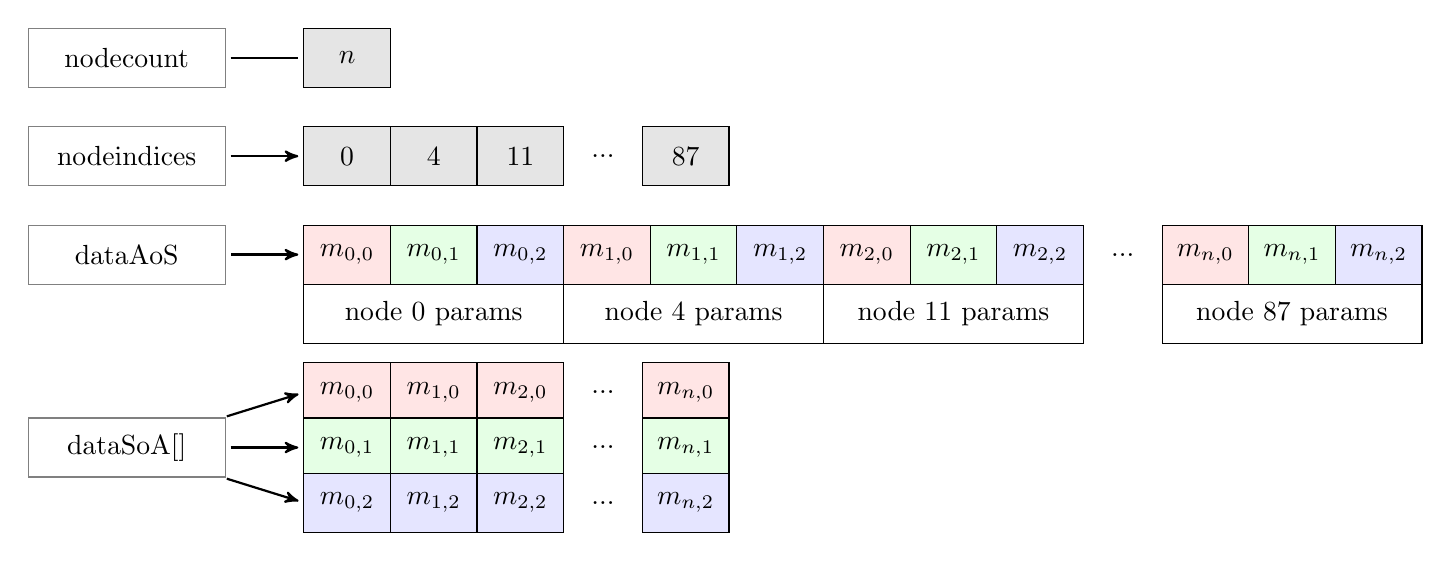
\begin{tikzpicture}[x=0cm, y=0cm, node distance=0 cm,outer sep = 0pt]
\tikzstyle{t0}=[draw, rectangle,  minimum height=\nodeheight, minimum width=\nodewidth, fill=red!10,anchor=south west]
\tikzstyle{t1}=[draw, rectangle,  minimum height=\nodeheight, minimum width=\nodewidth, fill=green!10,anchor=south west]
\tikzstyle{t2}=[draw, rectangle,  minimum height=\nodeheight, minimum width=\nodewidth, fill=blue!10,anchor=south west]
\tikzstyle{t3}=[draw, rectangle,  minimum height=\nodeheight, minimum width=\nodewidth, fill=yellow!20,anchor=south west]
\tikzstyle{index}=[draw, rectangle,  minimum height=\nodeheight, minimum width=\nodewidth, fill=black!10,anchor=south west]
\tikzstyle{blank}=[draw=none, fill=none, rectangle,  minimum height=\nodeheight, minimum width=1cm, anchor=south west]
\tikzstyle{over}=[draw=black, rectangle,  minimum height=\nodeheight, minimum width=3.3cm, anchor=south west]
\tikzstyle{pointer}=[draw=black!50, rectangle,  minimum height=\nodeheight, minimum width=2.5cm, anchor=south west]

\node[pointer] (dataAoS) at (0,0)         {\lst{dataAoS}};
\node[t0] (m00) [right = 1cm of dataAoS] {$m_{0,0}$}
    edge[pil,<-] (dataAoS.east);
\node[t1] (m01) [right = of m00] {$m_{0,1}$};
\node[t2] (m02) [right = of m01] {$m_{0,2}$};
\node[over] (over0) [below = of m01] {node 0 params};
\node[t0] (m10) [right = of m02] {$m_{1,0}$};
\node[t1] (m11) [right = of m10] {$m_{1,1}$};
\node[t2] (m12) [right = of m11] {$m_{1,2}$};
\node[over] (over1) [below = of m11] {node 4 params};
\node[t0] (m20) [right = of m12] {$m_{2,0}$};
\node[t1] (m21) [right = of m20] {$m_{2,1}$};
\node[t2] (m22) [right = of m21] {$m_{2,2}$};
\node[blank] (blank) [right = of m22] {...};
\node[over] (over2) [below = of m21] {node 11 params};
\node[t0] (m30) [right = of blank] {$m_{n,0}$};
\node[t1] (m31) [right = of m30] {$m_{n,1}$};
\node[t2] (m32) [right = of m31] {$m_{n,2}$};\\
\node[over] (over3) [below = of m31] {node 87 params};

\node[index] (i0) [above = 0.5 cm of m00]   {$0$};
\node[index] (i1) [right = of i0]   {$4$};
\node[index] (i2) [right = of i1]   {$11$};
\node[blank] (blanki) [right = of i2] {...};
\node[index] (in) [right = of blanki]   {$87$};
\node[pointer] (indicesAoS) [left = 1cm of i0]   {\lst{nodeindices}}
    edge[pil,->] (i0.west);

\node[index] (nnodes) [above = 0.5 cm of i0]   {$n$};
\node[pointer] (numnodes) [left = 1cm of nnodes]   {\lst{nodecount}}
    edge[pil,-] (nnodes.west);

\node[t0]  (00) [below = 1 cm of m00] {$m_{0,0}$};
\node[t0]  (10) [right = of 00] {$m_{1,0}$};
\node[t0]  (20) [right = of 10] {$m_{2,0}$};
\node[blank] (blank0) [right = of 20] {...};
\node[t0]  (n0) [right = of blank0] {$m_{n,0}$};

\node[t1]  (01) [below = 1.7 cm of m00] {$m_{0,1}$};
\node[t1]  (11) [right = of 01] {$m_{1,1}$};
\node[t1]  (21) [right = of 11] {$m_{2,1}$};
\node[blank] (blank1) [right = of 21] {...};
\node[t1]  (n1) [right = of blank1] {$m_{n,1}$};

\node[t2]  (02) [below = 2.4 cm of m00] {$m_{0,2}$};
\node[t2]  (12) [right = of 02] {$m_{1,2}$};
\node[t2]  (22) [right = of 12] {$m_{2,2}$};
\node[blank] (blank2) [right = of 22] {...};
\node[t2]  (n2) [right = of blank2] {$m_{n,2}$};

\node[pointer] (indicesSoA) [left = 1cm of 01]   {\lst{dataSoA[]}}
    edge[pil,->,anchor=east] (00.west)
    edge[pil,->] (01.west)
    edge[pil,->] (02.west);

\end{tikzpicture}

\caption{The current AoS layout of mechanism parameters for all applicable nodes.}
\end{figure}
%------------------------------------------------------------------

\noindent
Observations
\begin{itemize}
\item
    Splitting the cells into seperate, thread-specific, data structures complicates the code. This feels like it was added at some point to facilicate threading.
\item
    Could be stripped away, to store all cells on a node/numa-region/device into a single pool.
\item
    The AoS storage is inefficient:
    \begin{itemize}
    \item
        It doesn't vectorize (see \fig{fig:papisample}).
    \item
        Poor cache/bandwidth utlization for loops (such as the \lst{jacob} update) where only one or two data values in a mechanism are touched. For each 64 byte cache line loaded, only 8 bytes of 64 are used.
    \end{itemize}
    An SoA storage would address both issues.
\item
    With SoA vectorization of most loops would still not be possible, because of the gather/scatter implicit in using the node indexes to read/write to the V and RHS vectors.
    \begin{itemize}
    \item
        Perform scatter before computing the current, then gather after.
    \end{itemize}
\end{itemize}

